\section{Einleitung}

Struktur: Form $\rightarrow$ Funktion\\
Funktion folgt Form, Form folgt Sequenz\\
Proteine, RNA, DNA: Sequenzen\\
\\
\underline{4 Strukturlevels:}
\begin{itemize}
	\item primäre Struktur (Sequenz): 1 Dimension
	\item sekundäre Struktur (grobe Annäherung an Struktur): 2 Dimensionen
	\item tertiäre Struktur (räumliche Struktur): 3 Dimensionen
	\item quartiäre Struktur (räumliche Anordnung von interagierenden Strukturen): 4 Dimensionen
\end{itemize}

Behandlung hauptsächlich 2D\\

% 
\subsection{RNA}\footnote{\url{https://de.wikipedia.org/wiki/Ribonukleins\%C3\%A4ure}}
Funktion:
\begin{itemize}
	\item Informationsträger
	\item Regulator/Katalysator
	\item Theorieder RNA-World
\end{itemize}

 - Nicht-Messenger-RNA: ncRNA (nc - non-coding)\\

\begin{itemize}
	\item Aufbau: Zucker-Phosphat-Rückgrat
	\item Basen:
	\begin{itemize}
		\item Purine: Adenin, Guanin
		\item Pyrimidine: Cytosin, Uracil
	\end{itemize}
	\item Paarung: A-U, G-C
	\item RNA einzelsträngige A-Helix (DNA: doppelsträngige B-Helix)
\end{itemize}

\subsection{R/DNA-Sekundärstruktur}
\underline{Definition:} Liste von Basenpaaren, sodass gilt (theoretische Regeln):
\begin{enumerate}
	\item erlaubte Basenpaarungen:
	\begin{itemize}
		\item Watson-Crick: AU, UA, GC, CG 
		\item Wobble: GU, UG
	\end{itemize}
	\item zwischen miteinander paarenden Basen müssen mindestens 3 Basen stehen
	$if(i,j) \epsilon B \rightarrow i < j-3 $\\
	Beispiel Paarung A und U:
	\begin{tabular}{cccccccc}
  		A & U & \underline{A} & U & A & U & A & \underline{U}\\
  		  &   &   & 1 & 2 & 3 & 4 &  \\
 	\end{tabular}
	\item keine Tripletts (Multipletts): eine Base paart maximal mit einer anderen
	$if(i,j);(i,k) \epsilon B \rightarrow j=k $
	\item keine pseudo-Knoten: Basen kreuzen sich nicht
	$if(i,j);(k,l) \epsilon B \rightarrow i<j<k<l\ und\ i<k<l<j $
\end{enumerate}

\underline{Motivation zu Regeln:} jedes Basenpaar teilt das Molekül in 2 Teile (innen und außen), die miteinander \underline{nicht} interagieren (vor allem Regel 3 + 4)
\\\\
physikalische Eigenschaften:
\begin{enumerate}
	\item Großteil des stabilisierenden Energie für RNA-Struktur kommt aus der Sekundärstruktur
	\item Sekundärstruktur bildet sich zeitlich vor Tertiärstruktur aus
\end{enumerate}

Experimenteller Nachweis 3D, 4D:
\begin{itemize}
	\item Röntgenkristallographie: Kristall benötigt $\rightarrow$ oft schwierig
	\item nuclear magnet resonanz (nmr): stark konzentrierte Lösung benötigt, nur Distanzen zwischen Atomen ermittelbar
\end{itemize}

\underline{für 2D:} Methoden, die bevorzugt einzelsträngige oder doppelsträngige Strukturen schneiden

\subsection{Strukturabbildungen}
\begin{enumerate}
	\item Strukturplot:\\
	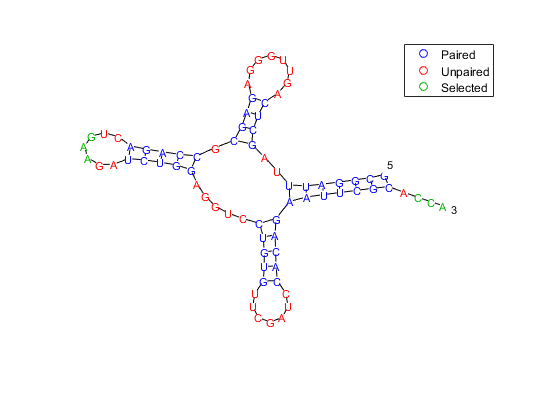
\includegraphics[width=0.8\textwidth]{lectures/160404/pix/structure.png}
	\item Dot-Bracket:\\
	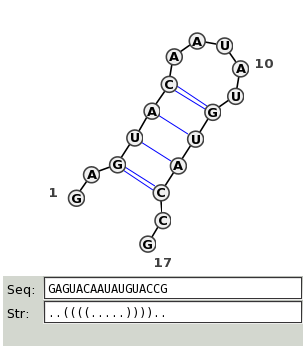
\includegraphics[width=0.7\textwidth]{lectures/160404/pix/dot_bracket.png}
	\item Zirkulärplot:\\
	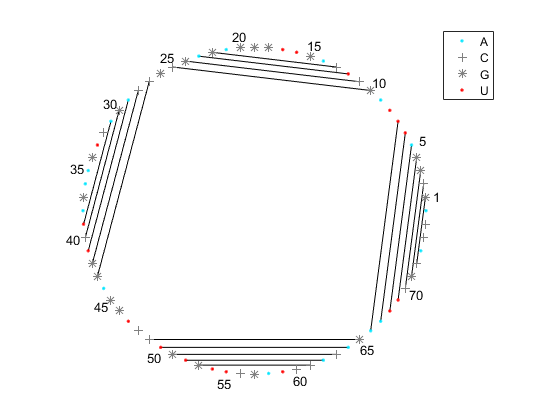
\includegraphics[width=0.95\textwidth]{lectures/160404/pix/circular_plot.png}
	\item Bogenplot:\\
	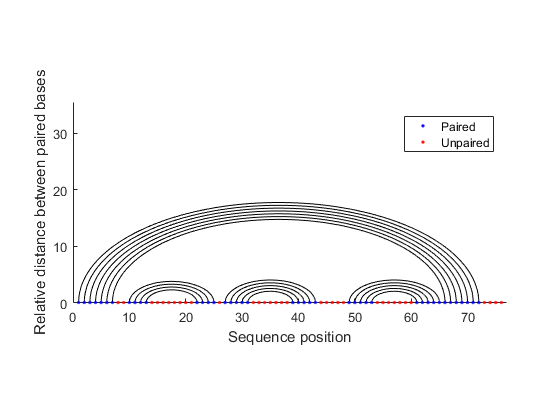
\includegraphics[width=0.95\textwidth]{lectures/160404/pix/arc_plot.png}
	\item Mountainplot:\\
	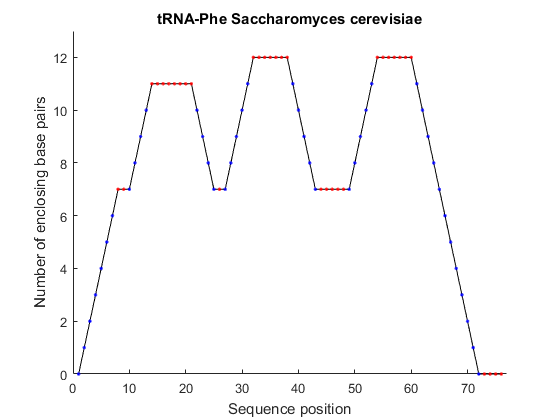
\includegraphics[width=0.8\textwidth]{lectures/160404/pix/mountain_plot.png}
	\item Dotplot:\\
	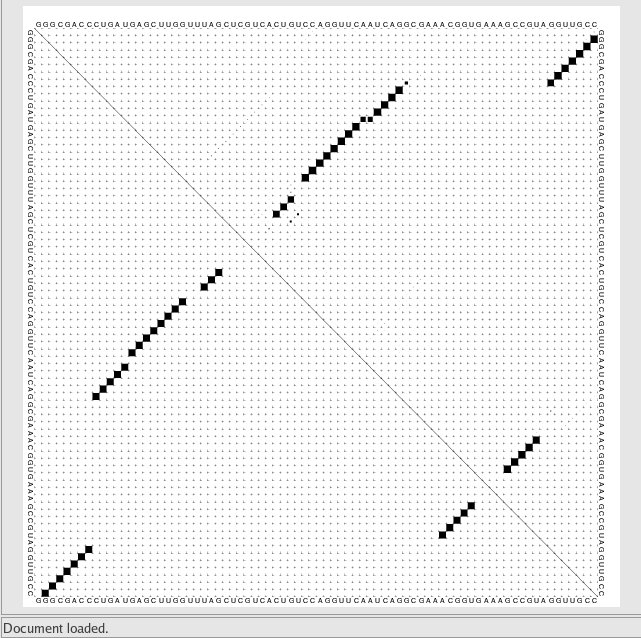
\includegraphics[width=0.8\textwidth]{lectures/160404/pix/Dotplot.jpg}
\end{enumerate}

\section{Strukturvorhersage}
\begin{itemize}
	\item durch Aufteilung kann Dynamics Programming verwendet werden
	\item Beginn: einzelne Basen $\rightarrow$ keine Struktur
\end{itemize}

\subsection{Nussinov}
 - von Ruth Nussinov (1978)\\
 - Versuch Struktur mit der maximalen Anzahl der Basenpaare zu finden (Grundlage ist Sequenz)
\\\\
\underline{Dynamics Programming}\\
\textbf{ - Initialisierung:}
\begin{itemize}
	\item $N(i,i) = 0$
	\item $N(i,j)=0\ if\ i<j\le i+3$ (siehe Regel 2)
	\item $N(j+1, j) = 0$
\end{itemize}
\textbf{- Brechnung:}\\
$N(i,j)=max \begin{cases}
               N(i+1, j)\ (ungepaart)\\
               \displaystyle\max_{i+3<k \le j}\ N(i+1, k-1) + N(k+1, j) + F(i,k)\\
\end{cases}$
\\\\\\
mit $F(i,k)= \begin{cases}
               1\ if\ i,k\ \epsilon\ \{AU, GC, GU\}\\
               -\infty\ else\\
\end{cases}$
\\\\\\
Basenpaarung mit i und k teilt Sequenz in inneren und äußeren Teil:\\
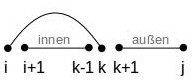
\includegraphics[width=0.3\textwidth]{lectures/160404/pix/pairing.jpg}
\\
$\rightarrow$ höchste Punktzahl wahrscheinlichste Sekundärstruktur
\\\\
Resourcenbedarf:
\begin{itemize}
	\item Speicher: $\mathcal{O}(n^2)$
	\item Prozessor: $\mathcal{O}(n^3)$
\end{itemize}